\section{Literature Review}
Computational Fluid Dynamics (CFD) is a broad term encompassing a number of different numerical methods and technique to solve fluid flow problems. CFD provides a practical alternative to physical models where analytical solutions are impossible or unknown. As such CFD is widely employed by industry and there are an estimated 250,000 purely CFD related jobs worldwide and an estimated potential market value of 2.9 Billion (\cite{hanna_parry}). 
\\\\
Whilst CFD formally existed as an area of research as early as the 20's, major developments and the formative years of the subject are accountable to increased efforts during the cold war. Large increases in government funding accelerated CFD development motivated by the desire to improve missile technology \cite{hanna_parry}. As such these development mainly focused on improvements in understanding of supersonic aerodynamics and combustion phenomena (\cite{scientific_computing_world_2017}). Being subject to large government funding, notable developments in CFD, such as the "Particle-In-Cell" method stem from the work of Harlow and his team, T3, at the Los Alamos National Laboratory, a continuation of the Manhattan Project. These initial developments ran on supercomputers (\cite{harlow_2003}), making them prohibitively expensive to most industrial and academic applications, hence work on the subject through the 60's and early 70's is most entirely military based.
\\\\
As the cost of computing power decreased and hence its accessibility increased, more varied applications and methods were introduced. Breakthroughs in CFD starting in the mid 70's going through the 80's are still in use and recognizable to anyone familiar with the subject, two notable exams are the k-epsilon turblence model described by Launder and Spalding in their 1974 paper "The numerical computation of turbulent flows" (\cite{launder_spalding_1974}) and the SIMPLE scheme proposed by Spalding and Patankar in their paper "A calculation procedure for heat, mass and momentum transfer in three-dimensional parabolic flows" (\cite{patankar_spalding_1972}). Incidentally it is Patankars book on Finite Volume methods "Numerical Heat Transfer and Fluid Flow" that is credited with popularizing the Finite difference and Volumes methods, notably due to their ease to program and wide applicability \cite{hanna_parry}. Programs spawned from this are still around, notably FLUENT and STAR-CD.
\\\\
The finite difference and volumes methods pioneered during this era are still the most widely employed tools used. They represents mesh based CFD methods where the spatial domain is discretized into  grid segments and  a series of equations formed at cell faces. This gives rise to two classifications of CFD techniques, mesh and mesh free. Mesh based CFD methods differ from Meshfree methods in that they provide a Eulerian description of the flow field. In a Eulerian description a specific location is observed and the flow at this given location is seen to evolve as time passes. In a Lagrangian description of a flow a certain parcel of fluid is observed and its position is also seen to evolve with time. In practice the difference between the two descriptions are exhibited in the use of either a grid based or particle based simulation. However each poses further specific advantages, particle based simulations exhibit less numerical diffusion and naturally apply continuity. 
\\\\
However major differences are exhibited in the way they are calculated. Mesh based simulations assemble a large matrix of simultaneous linear equations which are solved via an iterative method. However, for example, the DVM developed as part of this project, the calculation of the velocity of each particle is independent of each other (the equations are not simultaneous). Hence there are significant differences in their implementation. This leads to some approaches being more ideal for calculations on parallel rather than serial computing architectures.
\\\\
As the availability of computing power increases, so does the scope of what may be achieved, this has led to increasing interest in real-time simulation. The development of Real-Time CFD has mainly been motivated for non-engineering related applications. Primarily for use in video games and special effects, both applications requiring results that look good, rather than provide accurate results. Coupled with the development of GPU's, an extensively parallel computing architecture, a number of realtime fluid simulations have emerged. The most notable of these being Nvidia Flex, a game physics engine. As the performance and accuracy of these simulations increase their scope as use as engineering tools likewise increases.
\\\\
Real-Time simulation posses possible innovation in many engineering sectors. For example it streamlines the design process by eliminating the wait time between creating a CFD model and the results from the calculations. This represents a shift from iterative based design to interactive design. However the uses of a real-time engineering grade simulation posses innovations more far reaching than the engineering process itself. For example Work at the University of Leeds has successfully implemented a real-time CFD simulation of the heat generated in a data centre and implemented implemented a predictive active cooling system based on this (\cite{khan_delbosc_noakes_summers_2015}). This example is notable and unique in that a system utilizing Real-Time CFD has been implemented. There are numerous other areas that development of Real-Time CFD poses advantages in, for example simulation of surgery \cite{c4c8c2aa4eea4ba190da55f77965537b}, contaminant spread and control, 
\\\\
The method of CFD chosen to develop a Real-Time CFD code must achieve a level of performance adequate to obtain it's real time objective. Combined with the increase in potential performance offered by code running on a parallel architecture compared to a serial architecture for the same cost, the popularity of methods utilizing a Lagrangian description of the flow field have become popular. The two most prominent of these being the Lattice-Boltzmann Method and Smoothed Particle Hydrodynamics. 

\begin{figure}[H]
\begin{center}
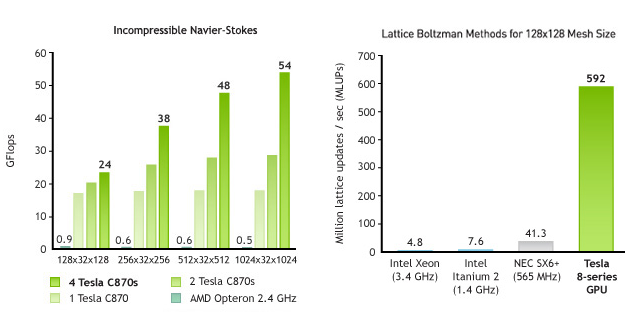
\includegraphics[width=1.0\textwidth]{Referenced_Figures/CPUGPU-Comparison.png}
\caption{\label{fig:GPUCPUCOMP}Distant Elements Approximated to a Single Cluster}
\end{center}
\end{figure}

Figure \ref{fig:GPUCPUCOMP} shows the results of an investigation by Nvidia into the performance of both Finite-Volumes (left) and Lattice-Boltzman (right) running on a selection of CPU's and GPU's (\cite{computational_fluid_dynamics_nvidia}). It is pertinent to note the author of this study, Nvidia, manafature GPU units and as such have a vested interest in the subject. Further, there is important data omitted from the study, namely the number of cores that each CPU unit is running on is not mentioned. Assuming the worst case scenario and each CPU is running on a single core out of a possible 4, and as such the CPUs tested can actually run four times as fast, the conclusions remain the same. There is a decrease in computational time by performing the simulation on the GPU, however the important comparison is the far larger decrease present in using a GPU for the Lagrangian method (Lattice-Boltzmann) over the Eulerian method (Finite-Volumes). 
\\\\
This does not demonstrate that the use of the Lattice-Boltzmann method necessarily represents a performance increase (the price of the CPU and GPUs are not taken into account), rather its conclusions are limited to demonstrating that the Lattice-Boltzmann method is more suited to performing calculations on a parallel architecture relative to the Finite-Volumes method. Figure \ref{fig:GPUCPUPERF} shows the performance in FLOPS (Floating Point Operations) of an average CPU versus and average GPU corrected for price, the graph is taken from the article "Acceleration of a 3D Euler Solver Using Commodity
Graphics Hardware" (\cite{brandvik_pullan_2008}). A substantial difference is seen to develop after 2003 and the trend continues resulting in a substantial (around a magnitude of difference) between the parallel and serial architectures. This puts into context the advantage of a method of CFD that may be programmed for a parallel naturally poses. This trend also explains the recent increased interest in Real-Time CFD as the increase in available processing power increases the scope of a real-time simulation.

\begin{figure}[H]
\begin{center}
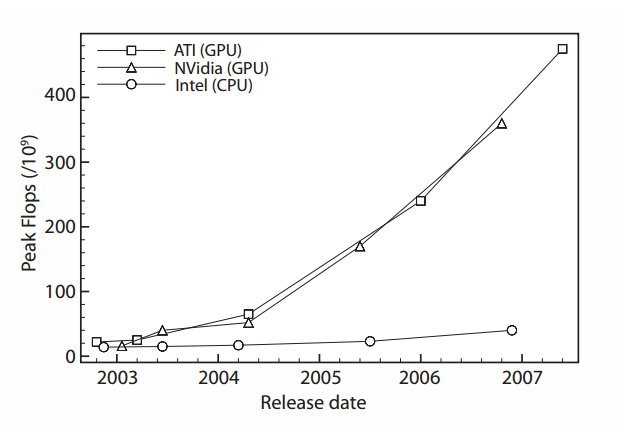
\includegraphics[width=0.7\textwidth]{Referenced_Figures/CPUGPU-Performance.png}
\caption{\label{fig:GPUCPUPERF}Distant Elements Approximated to a Single Cluster}
\end{center}
\end{figure}

The Lattice-Boltzmann method (LBM) is unique from other methods of CFD discussed here, firstly because it does not solve the Navier-Stokes equations and secondly as it is designed specifically to be implemented on parallel computing architectures. The LBM uses a series of particles that represent groupings of molecules and their interactions are modelled. As the LBM simulates molecular interactions it does not rely upon the assumptions that Navier-Stokes based methods such as Finite-Volumes makes in order for continuum conditions to apply. Hence it can be applied in situations where continuum assumptions do not apply. This has made the LBM especially important in work on microfluidics (where the flow has a Knudsen Number of less than 0.1) and medical simulations (where multiphase flows are present) (\cite{c4c8c2aa4eea4ba190da55f77965537b})
\\\\
Smoothed Particle Hydrodynamics (SPH)
\\\\
Discrete Vortex methods are a class of Lagrangian methods, they indirectly solve the Navier-Stokes equation by considering the vorticity of particles and determining the velocity field induced (\cite{cottet_koumoutsakos_2008}). Their implementation is discussed further in section, however being a Lagrangian method they are programmed easily for parallel architectures. Vortex methods however have not seen the same interest as SPH or LBM.
\\\\
Rosenhead was the first to formulate a complete vortex method (\cite{rosenhead_1931}) for 2D, inviscid and incompressible flow. However Further developments to vortex methods have extended their capability to include compressible flows (\cite{ELDREDGE2002371}), viscous flows (\cite{BADEN1990278}), turbulent flow (\cite{barba_1996}) and even combustion (\cite{Lakkis2003435}) making them a robust choice for simulation of many phenomena. However their major disadvantage is their inability to model strong boundary layer interactions such as pipe flows. However plenty of examples exist for simpler situations such as the flow around a sphere (\cite{johnson_patel_1999}) or aerofoils (\cite{xu_1999}), these flows are characterised by a stationary solid body moving in a large body of fluid, producing a "free wake". This makes them an ideal for the wake regions produced by aircraft it flight, further is a simplistic model of lift is used such as a Horseshoe Vortex then solid bodies need not even be taken into account.
\\\\
In a Discrete Vortex Method a number of particles are assigned initial positions and vorticity, the operating loop of the simulation can then be summarized as follows; the velocity field at every particle is determined, each particle is then iterated to a new position using the value of the velocity field and the new value of the velocity field calculated and the procedure repeated. The calculation of the velocity field requires the consideration of the vorticity of every other particle, and this is required to be considered for every particle, hence the complexity of a vortex method increases proportional to $N^2$ where $N$ is the number of particles. This is known mathematically as an N-Body problem and occurs predominantly in astrophysics.
\\\\
Vortex methods have traditionally incorporated a semi-Lagrangian method using Harlows previously mentioned "Particle-In-Cell" method, this was done so that viscous effects may be calculated through vortex stretch (\cite{liu_2001}). However grid free methods purely Lagrangian formulations of vortex methods have since been developed that take into account viscous effects (\cite{barba_1996}). Purely Lagrangian formulations benefit in that they closely emulate the maths of their astrophysics N-Body problem counterparts.
\\\\
The comparison between the N-Body encountered in astrophysics and Vortex methods is not trivial. In astrophysical problems a series of planets (analogous to vortex particles) are present and the gravitation of every planet effects the velocity of every other plane, whereas in Vortex methods the velocity of every particle is dependant on the vorticity of every other particle. The gravitational field decays according to an inverse square law and the influence of the vorticity of a particle decays with an inverse cube law.  Astrophysical N-Body problems have a wealth of research and established methods of optimization, due to the similarities between the two problem formulations these methods of optimization may pose the possibility of being adapted to vortex methods.
\\\\
A common algorithm used to optimize the simulation of an N-Body problem is the Barnes-Hut simulation, presented by Dr. Josh Barnes and Dr. Piet Hut in their paper "A hierarchical O(N log N) force-calculation algorithm" (\cite{barnes_hut_1986}). Figure \ref{fig:BarnesHutSpace} is taken from Barnes and Hut's original paper and shows how the spatial domain is segmented into discrete partitions

\begin{figure}[H]
\begin{center}
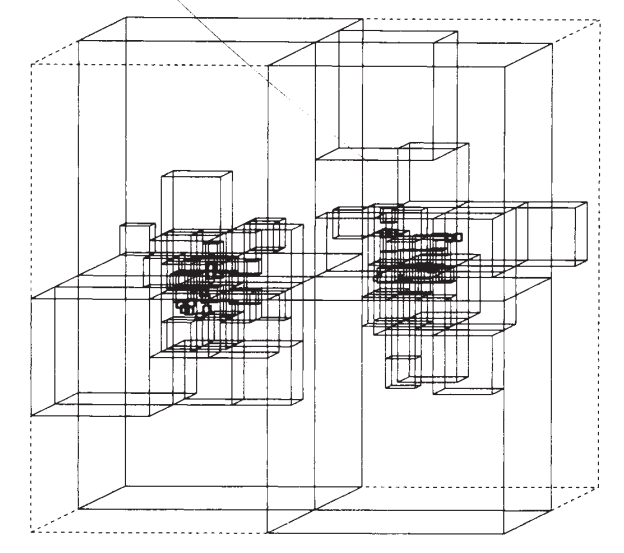
\includegraphics[width=0.7\textwidth]{Referenced_Figures/BarnesHutSpace.png}
\caption{\label{fig:BarnesHutSpace}Distant Elements Approximated to a Single Cluster}
\end{center}
\end{figure}

Planets within these partitions are assumed to act as one planet of increased strength and an equivalent position. By assuming a number of planets can be assumed to act as one planet less calculations are performed, and hence calculation time decreased. Further, these spatial segments of planets can be segmented together numerous times. These methods are known as Influence Tree Methods.The theory behind this is perfectly applicable to Vortex Methods. However a number of modifications can be made to exploit features of Vortex Methods. The discrete particles in a DVM are distributed over a vortex sheet, whilst the sheet itself takes a 3d form there may be potential optimization potential by segmenting the spatial domain based up a 2d representation of this sheet. This report aims to implement a novel modification of the Barnes Hut algorithm applied to vortex methods.

\subsection{Concluding Remarks}
Early years in the development of CFD led to the development of many varied approaches to simulation, however the Finite Volume method has become the most successful and widely deployed method. However with increased computing power offered from parallel architectures such as GPUs there has been renewed interested in the methods developed before the Finite Volumes method took prevalence. The methods that have seen renewed interest employ either a particle or statistical mechanics approach, these approached can be programmed naturally for parallel architectures whilst the mesh based Finite Volumes method do not.
\\\\
The Lattice Boltzman and Smoothed Particle Hydrodynamic methods have become the most popular choices for Real-Time CFD simulation, Vortex methods have not seen the same interest and development, however their mathematical implementation represents an N-Body problem. N-Body problems occur in Astrophysics problems and have been subject to research and optimization methodologies have been developed. This report aims to develop a Discrete Vortex Method Simulation optimized using two methodologies widely applied to Astrophysical N-Body problems however implemented in the context of a vortex Wake simulation. 
\\\\
%Info to write about: vorticity Vs. velocity variables, bring particle in cell back in context, used in vortex methods but introduces unacceptable innacuracies
%http://www.jstor.org/stable/95835?seq=17#page_scan_tab_contents:Reference for not using explicit scheme from rosenhead
%https://books.google.co.uk/books?id=WsjzOcEHmkMC&pg=PA2&lpg=PA2&dq=rosenhead+vortex&source=bl&ots=cjbRcAkTzg&sig=WHcsAJbu57LL4-3Z1VkwoWK6sOo&hl=en&sa=X&ved=0ahUKEwi267v20L3TAhVEQBoKHVyYB5UQ6AEITzAH#v=onepage&q=rosenhead%20vortex&f=false:book with good vortex methods intro
